\newcommand{\texCommand}[1]{\texttt{\textbackslash{#1}}}%

\newcommand{\exemplo}[1]{%
\vspace{\baselineskip}%
\noindent\fbox{\begin{minipage}{\textwidth}#1\end{minipage}}%
\\\vspace{\baselineskip}}%

\newcommand{\exemploVerbatim}[1]{%
\vspace{\baselineskip}%
\noindent\fbox{\begin{minipage}{\textwidth}%
#1\end{minipage}}%
\\\vspace{\baselineskip}}%


Este capítulo busca elucidar conceitos importantes para o entendimento do trabalho, partindo de uma melhor descrição da COVID-19 iniciada na introdução, assim como suas políticas públicas e o seus impactos em diversas regiões. Bem como um conceitos essenciais sobre modelagem espacialmente explícitas utilizando-se software de modelagem multiagente.
\todo{Seguindo a partir disso apresentar no capitulo 2.1 Contextualização do COVID-19. 
Capitulo 2.2 Descrição sobre Epidemiologia e sua atuação na COVID-19. Capitulo 2.3 Conceitos de modelos e de modelagem baseada em agentes. 2.4 Abordagem do geoprocessamento, ferramentas QGIS e OpenStreetMap. 2.5 Simulação Computacional e aprendizagem didáticas com simulações. 2.6 Introdução da linguagem Gama. 2.7 Ferramenta de modelagem COMOKIT. 2.8 Falta completar o roadmap, descrevendo as subseções}

%%%%%%%%%%%%%%%%%%%%%%%%%%%%%%%%%%%%%%%%%%%%%%%%%%%%%%%%%%%%%%%%%%%%%%%%%%%%%%%%
%%%%%%%%%%%%%%%%%%%%%%%%%%%%%%%%%%%%%%%%%%%%%%%%%%%%%%%%%%%%%%%%%%%%%%%%%%%%%%%%
%%%%%%%%%%%%%%%%%%%%%%%%%%%%%%%%%%%%%%%%%%%%%%%%%%%%%%%%%%%%%%%%%%%%%%%%%%%%%%%%
\section{COVID-19}

\subsection{A Pandemia da COVID-19}

A Organização Pan-Americana da Saúde (OPAS) publicou que em 31 de dezembro de 2019, a Organização Mundial da Saúde (OMS) foi alertada sobre casos de pneumonia na cidade de Wuhan, província de Hubei, na República Popular da China. A nova cepa, até o momento ainda desconhecida a seres humanos de coronavírus foi confirmada em janeiro de 2020.

Ao todo, sete coronavírus humanos (HCoVs) já foram identificados: HCoV-229E, HCoV-OC43, HCoV-NL63, HCoV-HKU1, SARS-COV (que causa síndrome respiratória aguda grave), MERS-COV (que causa síndrome respiratória do Oriente Médio) e o, mais recente, novo coronavírus (que no início foi temporariamente nomeado 2019-nCoV e, em 11 de fevereiro de 2020, recebeu o nome de SARS-CoV-2). Esse novo coronavírus é responsável por causar a doença COVID-19.

No Brasil, foi inicialmente declarado uma Emergência de Saúde Pública de Importância Nacional (ESPIN) de acordo com a Portaria Nº 188, de 3 de fevereiro de 2020 publicada no Diário Oficial da União, a portaria recomendou divulgar informações a população e até o momento não aplicou determinações restritivas para controle da COVID-19, chamada até a data da divulgação da portaria de  2019-nCoV.

De acordo com informações divulgadas pela Organização Pan-Americana da Saúde (OPAS), foi declarado em 11 de março de 2020 com objetivo de interromper a propagação do vírus uma Emergência de Saúde Pública de Importância Internacional (ESPII) – o mais alto nível de alerta da Organização.  


\subsection{O que são coronavírus}

Os coronavírus são uma família de vírus que possuem esse nome por conta das espículas na sua superfície que assemelham a uma coroa. Alguns sintomas vão desde resfriado leve, a síndrome respiratória aguda grave. Essa família começou a ser estudada em meados de 1960,  porém foi observado maior foco nesses vírus a partir de 2002 com o SARS (SARS-CoV), no qual essa nova variante era mais mortal e contagiosa do que as anteriores. 

\subsection{Tipos de coronavírus}

Atualmente são conhecidos 7 tipos de coronavirus que podem causar infecções respiratórias:

\begin{itemize}
\item Alfa coronavirus 229E e NL63;
\item Beta coronavirus OC43 e HKU1;
\item SARS-CoV;
\item MERS-CoV;
\item SARS-CoV-2.
\end{itemize}

\subsection{Impacto dos coronavírus }

Desses vírus já citados tanto os Alfa coronavirus quanto os Beta coronavirus já estavam presente no sociedade, porém seu impacto não é visto de forma tão alarmantes, pois seus sintomas estão associados a gripes comuns e problemas gastrointestinais como diarreias, náuseas e vômitos.

SARS-CoV (causador da Síndrome Respiratória Aguda Grave ou SARS), segundo a Organização Mundial da Saúde(OMS) foi a primeira nova doença grave e prontamente transmissível a surgir no século 21 e mostrou uma clara capacidade de se espalhar pelas rotas das viagens aéreas internacionais. O impacto dessa cepa foi notado ainda final de 2002 se espalhando por mais de 26 países e contaminando mais de 8000 pessoas até que foi totalmente controlada em julho de 2003, a Organização Mundial da Saúde definiu sua letalidade em torno de 3\%.

MERS-CoV (causador da Síndrome Respiratória do Oriente Médio ou MERS) gerou uma visibilidade internacional após em um surto em abril de 2012 na Arabia Saudita e diferente da SARS-CoV que foi controlada em menos de 1 ano, o MERS-CoV, segundo a Organização Mundial da Saúde, somente foi erradicado em fevereiro de 2022. Como pode ser observado na imagem abaixo \cite{WHOEMROM33:online}. 

O Novo Coronavirus inicialmente conhecido como 2019-nCoV começou a se propagar em Wuhan, na China no final de 2019 que posteriormente se espalhou pelo mundo, atingindo mais de 120 países (Ribeiro \& Silva, 2021).

O nome da doença foi posteriormente sugerido como COVID-19 pela Organização Mundial da Saúde(OMS). Algum tempo depois o Comitê Internacional de Taxonomia de Vírus denominou o vírus como SARS-CoV-2.

Segundo o Ministério da Saúde, o Brasil já ultrapassou os 30 milhões de pessoas que foram infectados desses mais de 29 milhões recuperados e mais de 660 mil óbitos. Além disso segundo a Organização Mundial da Saúde o número de infectados já ultrapassava 511 milhões de pessoas.

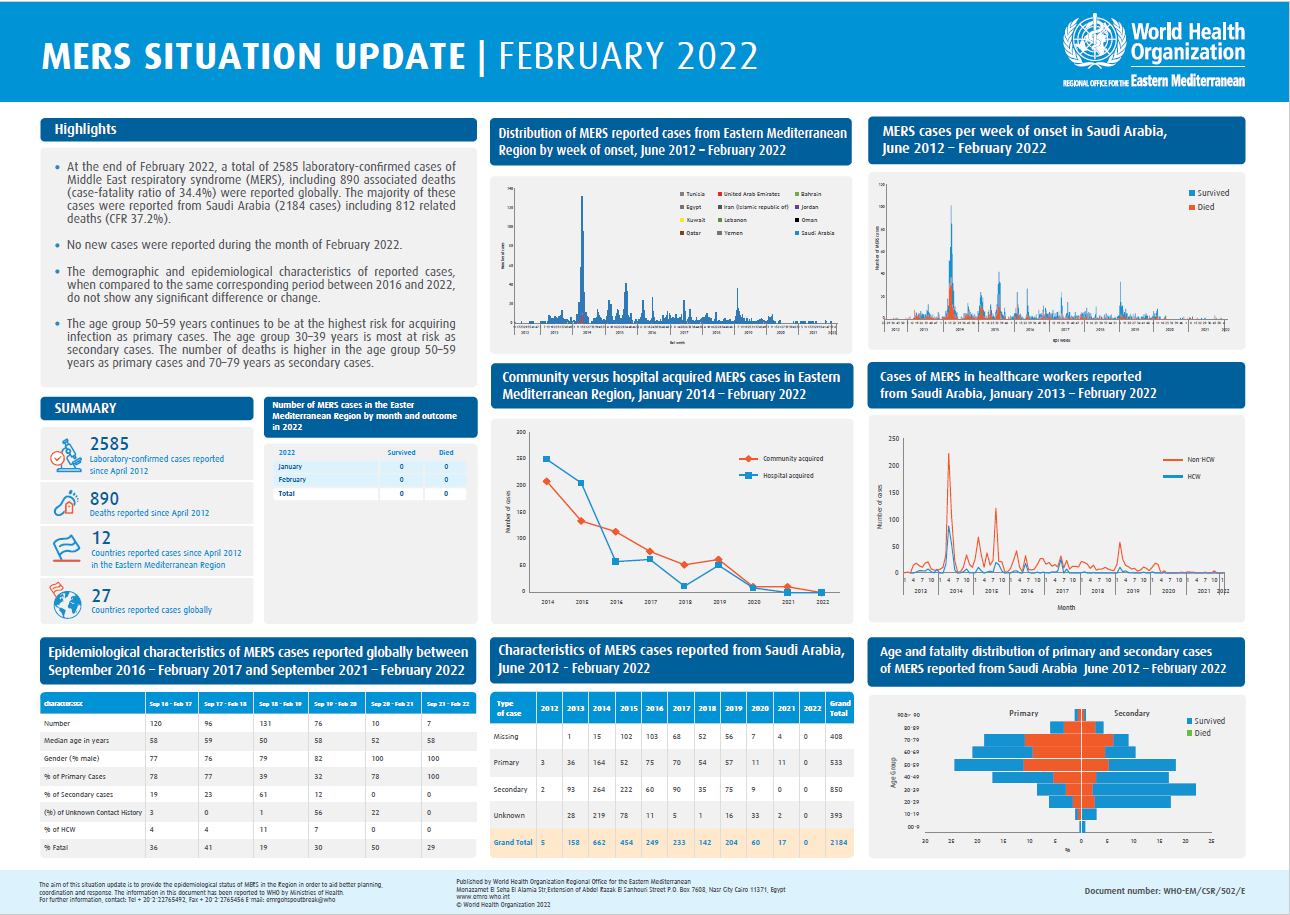
\includegraphics[width=15cm, height=15cm]{MERS.PNG}

\section{Epidemiologia}

\subsection{O que é Epidemiologia?}

Segundo Mark Woodward(2013) "epidemiologia é o ramo do estudo responsável por estudar as distribuições e os determinantes na população humana". Essas distribuições podem ser diversas como idade, profissão, classe social, histórico familiar, local geográfico, logo as distribuições não precisam ser baseadas necessariamente em espaço geográfico. Já os determinantes são fatores de risco que podem levar a infecção ou ao desenvolvimento do agente patológico, por exemplo herança genética, condições ambientais, exposição a pessoas contaminadas\cite{woodward2013epidemiology}. 

Leon Gordis(2013) define que os objetivos da atuação da epidemiologia são: Primeiro descobrir a origem da doença, assim como seus fatores de riscos e forma de transmissão. Segundo analisar o impacto que a doença causa na comunidade analisada. Terceiro estudar o grau de mortalidade das doenças, priorizando as que possui alta letalidade, em busca evitar complicações e aliar com tratamentos. Quarto utilizar novas medidas terapêuticas no tratamento das pessoas, analisando se os novos métodos obtiveram resultados melhores do que os antigos. Quinto se atentar a possibilidades de disseminação de novos problemas de saúde, por exemplo a disponibilização de novos produtos químicos no mercado para o consumo das pessoas\cite{gordis2013epidemiology}.  

A epidemiologia explora em grande parte, as populações de indivíduos em busca de pistas e soluções para sociedade, isso remete diretamente ao ramo da medicina, porém não se restringe somente a esse, possui também uma ligação forte com a estatística na sua analise de dados coletados e construções de gráficos. Quando é mencionado a analise de dados, também já é possível fazer uma associação com a computação. Isso demonstra que a relação dessa área de conhecimento com as demais ocorre por diversas frentes, onde cada um pode desempenhar um papel muito importante na construção de ações governamentais no auxilio da saúde da sociedade.

\subsection{Epidemiologia do COVID-19}

O COVID-19 possui características muito semelhantes ao do SARS-CoV, fato que é observado no trabalho de Zhou e colaboradores (2020) ao comparar o COVID-19 com coronavirus de encontrados em morcegos foi possível encontrar uma relação de 96\% de proximidade entre eles. Por conta disso suspeita-se que teve origem em morcegos passando posteriormente a algum animal intermediário que após sofrer mutações foi possível a transmissão para humanos (Nogueira e Silva, 2020), embora haja essas suspeitas ainda não foi encontrado esse animal intermediário. 

A propagação do COVID-19 já era especulado que seria também por gotículas presentes na fala, em tosses e espirros, contato pessoal próximo, como toque, abraço ou aperto de mão; contato com objetos ou superfícies contaminadas, seguido de contato com a boca, nariz ou olhos características que os outros coronavirus possuem na sua transmissão. Entretanto sua propagação é muito superior aos outros da sua família. Além disso, segundo a Organização Mundial da Saúde (OMS) embora o período de incubação do SARS-CoV possa ser de 2-10 dias, o do COVID-19 pode variar entre 5-12 dias, pode ser um agravante adicional para a propagação do vírus, pois como foi observado Zhengdong e colaboradores (2020) e também por BAI e colaboradores (2020) já estava ocorrendo casos de possíveis pacientes assintomáticos transmitindo o vírus em fevereiro de 2020.

Dentre o grupos de pessoas mais propensas a terem complicações estão as pessoas com comorbidades e idosos (Galvão e Roncalli, 2020). Esses grupos estão em uma situação de vulnerabilidade maior e possuem uma maior probabilidade de desenvolver a forma mais grave da doença e até levar a óbito, sobretudo dentro desses grupos é classificado como mais vulnerável ainda os idosos acima de 80 anos.

O que tornou o vírus potencialmente destrutivo não foi sua mortalidade que em um contexto geral, segundo os dados da Organização Mundial da Saúde, ficou em torno de 1.2\%, mas também a sua alta disseminação gerando assim uma superlotação dos leitos por pacientes com a síndrome respiratória aguda grave que é o quadro mais grave da doença, além disso existem problemas cardíacos, neurológicos, hepáticos e intestinais associados a doença. Ao gerar o colapso do sistema de saúde, pacientes inclusive com outras doenças não poderiam ser atendidos como foi o caso da Itália primeiro bimestre de 2020.

Formas de prevenção para o COVID-19 e outras doenças virais são cuidados com a higiene como lavar as mãos e uso de máscara principalmente em locais com grande aglomerações. As máscaras são o primeiro cuidado que pode ser tomada para evitar o contágio, mas não somente isso, como apontado por SINCLAIR e colaboradores (2020) diminui a probabilidade que as próprias pessoas infectadas possuem transmitir o viros, muitos profissionais de saúde que tem contato frequente com pessoas potencialmente iniciam seus turnos e ao longo desse desenvolve sintomas leves e continua trabalhando.    

\subsection{COVID-19 como pandemia}

Diante da crescente propagação do vírus no dia 30 de janeiro de 2020, a Organização Mundial da Saúde(OMS) declarou que o surto do novo coronavírus constitui uma Emergência de Saúde Pública de Importância Internacional (ESPII), essa medida é caracterizada como avançada no controle ao vírus que se propagava por diversos países. Tal medida somente pode ser feito pelo diretor-geral da OMS, após realizar uma reunião com especialistas os quais o orientam sobre medidas emergências e para barrar o crescente número de casos do vírus. Esse estado de emergência de Saúde Pública busca a cooperação global para reduzir os casos da doença.

No dia 11 de março de 2020 o diretor-geral da OMS anunciou que o COVID-19, passaria a ser caracterizado como uma pandemia que é um termo que gera muitas incertezas e preocupações internacionais. Devido a sua propagação por mais de 114 países e que pandemia é caracterizada com relação a distribuição geográfica pelo mundo  no momento do seu anúncio os casos já ultrapassavam 118 mil casos.

\section{Modelagem e Modelos}

\subsection{Modelos}

Um modelo é uma representação com um proposito de um sistema real no qual pode ser entendido como uma representação abstrata e mais simplificada de processos que ocorrem no mundo real, esses modelos buscam apresentar, analisar, compreender, explicar e até prever determinados fenômenos. O modelo é construído a partir da escolha dos parâmetros no qual o modelador analisa os dados e determina quais possuem um maior impacto na construção do modelo e quais dados são pouco relevantes para sua elaboração e construção, isso torna cada modelo essencialmente especial por ser construído por aspectos que o modelador acha relevante (Starfield ET AL. 1990) \cite{Qualitat24:online}. 

De outra forma pode ser entendido o modelo como uma representação de um sistema utilizando-se outro sistema com objetivo de facilitar o entendimento tanto por ser mais simples ou por possuir elementos mais conhecidos, além disso ambos apresentam funções semelhantes(Blackburn. 1997)\cite{blackburn}

\subsection{Modelagem de agentes e sistemas baseados em agentes}

A modelagem baseada em agentes (MBA) é uma metodologia usada para construir modelos formais de sistemas do mundo real que são compostos por unidades individuais que interagem repetidamente entre si e com seu ambiente.(Luis R. Izquierdo, Segismundo S. Izquierdo, William H. Sandholm. 2019)\cite{izquierdo2019introduction}. 

No entendimento de Bonabeau (2002), a MBA pode ser vista como conjunto de unidades autônomas que tomam suas decisões de forma individual baseadas em comportamentos, tais comportamentos são originados pela própria percepção sobre o ambiente e também sobre as interações geradas pelas outras unidades autônomas, essas unidades individuais podem ser chamadas de agentes. Esses podem ser capazes de evoluir, permitindo novos comportamentos e interações. Existe ainda a possibilidade da MBA utiliza-se de inteligencia artificial através de redes neurais, algoritmos evolucionários ou outras técnicas de aprendizado para permitir aprendizado e adaptações realistas\cite{bonabeau2002agent}. 

No mundo real assim como nas MBAs cada individuo desempenha um papel e suas interações individuais com outros e com o ambiente influenciarão o resultado que o grupo atingirá. A imagem abaixo mostra diversas interações entre pessoas e agentes computacionais.  


\figura{real_world}{Em um modelo baseado em agente, as unidades individuais do sistema do mundo real a ser modelado e suas interações são representadas de forma explícita e individual no modelo\cite{02Introd63:online}}{real_world}{width=0.75\textwidth}


As variáveis que moldam as interações entre os agentes assim como o comportamento desses agentes com o ambiente e com os demais indivíduos podem ser pensadas de forma mais simples ou elaboradas em contextos mais específicos ou complexos. Dessa forma pode-se observar também limitações na elaboração dos agentes e na construção modelo.

\subsection{Principais vantagens e desafios na Modelagem de agentes}

A modelagem baseada em agentes(MBA) possibilita observar certos comportamentos individuais de humanos e animais que não seriam possíveis distinguir corretamente em sistemas complexos, essa capacidade de analisar comportamentos individuais transforma a observação sobre um fenômeno em uma visão mais simplificada, alguns dos exemplos para esses comportamentos podem ser observados em epidemias, movimento de animais em grupos coordenados, trânsito de veículos. Além disso destaca-se a alta flexibilidade desses Sistemas Baseados em Agentes, uma vez que é possível fazer alterações tanto no ambientes, quantos nos agentes que interagem entre si. Conforme Bonabeau(2002) mesmo modelos simples baseado em agentes pode exibir padrões de comportamento complexos e contribuir com informações valiosas sobre a dinâmica do sistema do mundo real que ele emula \cite{bonabeau2002agent}

\figura{Passaros}{Movimento dos pássaros coordenados em bando}{Passaros}{width=0.75\textwidth}

Axtell (2000) Afirma que a modelagem baseada em agentes pode ser a solução para alguns processos levando a uma compreensão melhor sobre o comportamento do modelo, além de possibilitar melhores testes, permitindo a elaboração de suposições com isso possibilitando novas hipóteses desconhecidas anteriormente.\cite{Axtell:online}

Um desafio, comum a todas as técnicas de modelagem, é que o modelo deve ser construído num nível correto de descrição dos fenômenos, usando uma quantidade adequada de detalhes, para servir ao seu propósito. Outro desafio envolve a utilização da MBA nas ciências sociais, que geralmente envolvem seres humanos com comportamentos potencialmente irracionais, de escolhas subjetivas e psicologia complexa, aspectos difíceis de quantificar, calibrar e muitas vezes justificar. Outro desafio está relacionado à própria definição da MBA, a qual trata um sistema no nível de suas unidades constituintes, o que exige elevado poder computacional e tempo para simulação do modelo, conforme a escala e a complexidade modelada.

\section{Geoprocessamento e Sistema de Informações Geográficas}

\subsection{Geoprocessamento}

Geoprocessamento é a utilização de técnicas matemáticas e computacionais que tornam possível a realização de analises de informações geográficas, as quais são fundamentais em um pais igual ao Brasil. Além de ter um tamanho continental, carece de informações sobre as próprias características geográficas. Visando preservar a biodiversidade, conservar suas áreas prioritárias com potencialidades ecológicas, o Geoprocessamento é uma das tecnologias que tem sido utilizadas para preservar e proteger o território brasileiro.\cite{ximenes_modelagem_2008} \cite{georef:online}. 

As ferramentas que utilizam-se do Geoprocessamento são conhecidas como Sistemas de Informação Geográficas(SIG) ou Geographic Information System(GIS), podem ser entendidos como conjuntos de estruturas abrangendo programas computacionais, informações espaciais e hardwares possibilitando a analise e integração de diversos tipos de dados, criação de bancos, instituições, elaboração de mapas, documentos cartográficos\cite{Burrough:online}.

\figura{Geoprocessamento Imagem}{Componentes de um sistema de informação geográfica}{Geoprocessamento Imagem}{width=0.75\textwidth}



\subsection{Ferramenta de Sistema de Informações Geográficas QGIS}

Uma das ferramentas utilizadas na construção do trabalho foi o QGIS, seu nome tem origem em Quantum GIS (QGIS). Esse software faz parte do FOSS (Free and Open Source Software), logo uma das características marcantes do software é ser Código Aberto é gratuito\cite{Qgis:online} e pode ser baixado em diferentes sistemas operacionais como Linux, Mac, Windows. Além do mais conta com vários plugins desenvolvidos em varias linguagens sendo a principal Python. O software possui apoio da comunidade na construção e elaboração de projetos. Por fim dispõe de uma excelente integração com GAMA que foi a ferramenta principal utilizada na modelagem das simulações. 

O Qgis é um software livre para Sistema de Informação Geográfica, incubado pela Open Source Geospatial Foundation (OSGeo) e impulsionado por um grupo ativo de desenvolvedores voluntários que regularmente lançam atualizações e correções para os problemas verificados neste aplicativo. É utilizado em ambientes acadêmicos e profissionais, caracterizando-se por oferecer um número crescente de recursos nativos e “plugins” que podem ser desenvolvidos por qualquer usuário que saiba programar em C++ ou Python. Suporta uma ampla gama de formatos geoespaciais, tais como vetores, rasters e bases de dados. \cite{bruno2017aplicabilidade}
\subsection{OpenStreetMap}

O OpenStreetMap foi desenvolvido para criar um mapa livre editável do mundo. A ferramenta de mapeamento colaborativo Open Street Map (OSM) foi desenvolvida no ano de 2004, pelo estudante de computação Steve Coast, da University College London (UCL). Inicialmente, a ideia do projeto era realizar o mapeamento apenas da região do Reino Unido, mas logo despertou o interesse de pesquisadores de outros países do globo. \cite{ramm2011openstreetmap}.

Os mapas são criados usando dados de dispositivos portáteis de GPS, fotografias aéreas, de outras fontes livres ou simplesmente a partir do conhecimento local. O projeto foi iniciado porque a maioria dos mapas têm restrições legais ou técnicas para sua utilização, restringindo as pessoas de usá-los de forma criativa, produtiva ou outras formas alternativas. Ambas as imagens fundidas e o conjunto de dados vetoriais do OSM estão disponíveis para download sob uma licença Creative Commons Attribution ShareAlike 2.0 \cite{OpenStre2:online}.

Dados primitivos OSM são uma classe de objetos que podem serem armazenados via API no servidor. Os três tipos de suporte de dados são: \textit{Node}, \textit{Way} e \textit{Relation}. \cite{OpenStre2:online}

\begin{itemize}
\item Um nó é um par de coordenada de latitude/longitude. É usado como um bloco de construção para as outras características e como uma característica própria (pontos de interesse), para serem marcados, conforme necessário.
\item Um Caminho é uma lista de pelo menos dois nós que descrevem uma feição linear, tal como uma rua, ou similar. Os nós podem fazer parte de vários caminhos.
\item Uma relação é um grupo de zero ou mais com funções primitivas associadas. Ele é usado para especificar as relações entre objetos, e também pode modelar um objeto abstrato.
\end{itemize}

\section{Simulação Computacional}

A simulação computacional nos permite compreender um sistema complexo e tem sido empregada no auxílio à tomada de decisão \cite{Chung2003}.

Com o auxílio da simulação, podemos identificar e solucionar problemas de uma determinada região geográfica baseado em variáveis que influenciam os agentes e o meio que vivem. 

A modelagem e simulação baseada em agentes (ABMS) é um paradigma de simulação que utiliza agentes para analisar, reproduzir ou predizer fenômenos normalmente complexos e emergentes \cite{Klugl2012agent}. Na modelagem baseada em agente (ABM), um sistema é modelado como uma coleção de entidades autônomas de tomada de decisão chamadas agentes. Cada agente avalia individualmente sua situação e toma decisões com base em um conjunto de regras \cite{bonabeau2002agent}. A ABMS aplica o conceito de sistemas multiagentes para a estrutura básica de modelos de simulação, onde o sistema é modelado como
uma coleção de entidades autônomas de tomadas de decisão chamadas agentes \cite{macal2007agent}.

Um modelo representa uma simplificação da realidade e o processo de modelar envolve escolhas de níveis de abstração  e a linguagem utilizada para representação do modelo. 

Um sistema, que consiste em um grupo de agentes que podem potencialmente interagir uns com os outros, é chamado de Sistema multiagentes ou Multiagent system (MAS). Um MAS é composto por vários agentes que interagem ou trabalham em conjunto de forma a realizar um determinado número de tarefas ou objetivos. Esses objetivos podem ser globais do sistema, comuns a todos os agentes, ou individuais. Os agentes podem também assumir um comportamento colaborativo ou competitivo, dependendo da finalidade da aplicação com que o sistema multiagente foi designado.  Isto é, os tipos de agentes são definidos de acordo com o ambiente onde irão atuar. \cite{RosaSilvaMAS}

A modelagem baseada em agentes é agora uma abordagem popular para representar, estudar ou explorar sistemas geográficos complexos \cite{heppenstall2011agent}. Esta abordagem de modelagem se propõe a representar individualmente as entidades que compõem um sistema e suas interações, e permitir que  comportamentos macroscópicos surjam por simulação. A adoção de tal abordagem de modelagem foi muito estimulada pelo surgimento de plataformas de software cada vez mais poderosas, que agora permitem que modeladores sem um forte conhecimento em ciência da computação desenvolvam seus próprios modelos de maneira fácil e rápida. A tendência observada há alguns anos é o desenvolvimento de modelos muito mais descritivos integrando uma grande quantidade de dados, com uma representação detalhada do ambiente.
Apoiar o desenvolvimento de tais modelos requer o endereçamento de um conjunto de bloqueios científicos relacionados à integração de dados, eficiência de cálculo e visualização de simulações, que são particularmente desafiadores se a plataforma tiver que ser utilizável mesmo por cientistas que não são da computação. O GAMA (GIS Agent-based Modeling Architecture) foi desenvolvido para superar esses desafios. \cite{gamaplataform}.

\section{Gama}

O GAMA é um projeto open-source que passou por diversas melhorias de acordo com sua documentação, e hoje fornece uma linguagem acessível com tutoriais práticos para desenvolvimento de simulações. 

O paradigma da modelagem orientada a agentes dita que todo o “ativo” (entidades de um modelo, sistemas, processos, atividades, tais como, simulações e experimentos) pode ser representado como agente. Tendo isso em vista, o agente pode ser pensado como um componente computacional que apresenta seus próprios dados e executa seus próprios comportamentos, seja sozinho ou em interação com os outros agentes \cite{gamaplataform}. 

De acordo com a documentação técnica do GAMA, o software foi codificado em Java e utiliza uma linguagem GAML (Gama Modeling Language), uma linguagem orientada a agentes dedicada à definição de simulações baseadas em agentes e tem suas raízes em linguagens orientadas a objetos \cite{gamaplataform}.  


\subsection{Semântica Lexical de GAML}

A documentação técnica da Plataforma GAMA \cite{gamaplataform}, define que o papel do GAML é apoiar modeladores na escrita de modelos, que são especificações de simulações que podem ser executadas e controladas durante experimentos, especificados por planos de experimentos.

Devido ao paradigma orientado a objetos, um agente significa que tudo "ativo" pode ser representado como um agente. Em GAML (Gama Modeling Language), um agente pode ser representado como um componente computacional possuindo seu próprio dados e executando seu próprio comportamento, sozinho ou em interação com outros agentes. O uso de classes fornece as especificações para os objetos e os agentes são especificados por suas espécies, que lhes fornecem um conjunto de atributos, ações, comportamentos e também especifica propriedades de sua população , por exemplo, sua topologia ou cronograma \cite{gamaplataform}.

Qualquer espécie pode estar aninhada em outra espécie, o que é definido como macroespécie, caso em que as populações de suas instâncias serão obrigatoriamente hospedados por uma instância dessa macroespécie \cite{gamaplataform}. O conceito de herança e especialização estão presentes, semelhantes ao design orientado a objetos, as espécies podem herdar propriedades de outras espécies e possuir habilidades que são conjuntos de atributos e ações compartilhados entre diferentes espécies e herdados por seus filhos \cite{gamaplataform}.

As simulações e experimentos são definidos como duas espécies: modelo e plano de experimento. As relações entre espécies, modelos e planos de experimentos são codificados no metamodelo do GAML na forma de framework composto por três espécies abstratas que são os agentes, pai direto ou indireto de todas as espécies, modelo, o pai de todas as espécies que definem um modelo e experimento, pai de todas as espécies que definem um plano de experimento \cite{gamaplataform}.

Neste meta-modelo, as instâncias dos filhos do agente conhecem a instância do filho do modelo em que estão hospedados como seu mundo , enquanto a instância de plano de experimento identifica o mesmo agente como uma das simulações de que é responsável. O diagrama a seguir resume esse framework:

\figura{metamodelo_GAMA}{meta-modelo do GAML na forma de um framework }{metamodelo1}{width=0.75\textwidth}

A escrita de um modelo em GAML consiste na definição de um modelo na qual outras espécies, herdando diretamente ou não de um agente e representando entidades serão aninhadas com um ou vários planos de experimentos:

Ao executar um experimento no GAMA, é criado um agente de experimentos. O comportamento é especificado pelo plano de experimentos, responsável por criar agentes de simulação que os executará. Recursivamente, a inicialização de um agente de simulação criará a população de agentes das espécies definidas no modelo. Cada um desses agentes, ao serem criados, pode criar a população de sua microespécie \cite{gamaplataform}. 

\figura{metamodelo_and_usermodel_GAMA}{meta-modelo do GAML e modelo de usuário na forma de um framework }{metamodelo2}{width=0.75\textwidth}

\subsection{Organização de um modelo GAML}

Para realizar uma simulação em GAML devemos definir um modelo em GAML e posteriormente instanciar um agente modelo, que pode ou não conter microespécies.

A estrutura conceitual segue um padrão:

1. Definição de espécie global, precedida de um cabeçalho, para representar a espécie modelo;

2. Definição de microespécies;

3. Definição de planos de experimentos direcionados a este modelo.

\subsubsection{Cabeçalho do modelo}

O cabeçalho de um arquivo de modelo começa com a declaração do nome do modelo. Este nome é usado para construir o nome da espécie modelo nas quais as simulações serão instanciadas.

\figura{3_1_model}{declaração de um modelo}{basicmodel}{width=0.75\textwidth}

O exemplo acima criará uma espécie chamada \textit{dummy\underline{ }model}, filho da espécie abstrata model, a partir da qual as simulações serão instanciadas. 

A importação de um modelo pode ser realizada de duas formas: por herança ou importação direta. A imagem abaixo importa dois modelos por herança, ou seja, as declarações dos modelos importados serão mescladas na ordem de importação.

\figura{3_2_import}{importação de um modelo}{basicmodel}{width=0.75\textwidth}

A segunda forma de importação chamada de \textit{usage import } é reservado a \textit{micromodelos} e de acordo com a documentação técnica, está em fase experimental.

\figura{3_3_usage_import}{declaração da espécie global}{basicmodel}{width=0.75\textwidth}




\subsubsection{Declarações de espécies}

Uma espécie define seus atributos, ações e comportamentos, e por fim aspectos. Em Programação Orientada a Objetos, a espécie pode ser vista como uma classe e os agentes uma instância de uma espécie. 

A declaração da espécie global é única e não tem um nome específico. Ela representa um mundo, onde deve conter todos os atributos, ações e comportamentos globais.

\figura{3_4_global}{declaração da espécie global}{basicmodel}{width=0.75\textwidth}

As espécies regulares podem ser declaradas com o uso da palavra-chave \textit{species} e todas precisam ser renomeadas.

\figura{3_5_regular}{declaração de espécies regulares}{basicmodel}{width=0.75\textwidth}


\subsubsection{Declarações do experimento}

A declaração de experimentos começam com o uso da palavra-chave \textit{experiment} e contêm todos os parâmetros de simulação e a definição de saída que podem ser displays, monitores ou inspetores. 

\figura{3_6_experiment}{experimentos declarados}{basicmodel}{width=0.75\textwidth}

Existem quatro tipos de experimentos disponíveis no GAMA:

\begin{enumerate}
\item Experimento GUI que permite a exibição de uma interface gráfica com parâmetros de entrada e saída;
		
		\figura{3_7_gui_experiment}{experimentos declarados}{basicmodel}{width=0.75\textwidth}
		

\item Experimento em lote que perimte a execução de várias simulações sucessivas;

		\figura{3_8_batch_experiment}{experimentos declarados}{basicmodel}{width=0.75\textwidth}

\item Experimento de testes que permite a escrita de testes de unidade em um modelo para garantir a qualidade;

		\figura{3_9_test_experiment}{experimentos declarados}{basicmodel}{width=0.75\textwidth}

\item Experimento de memorização que permite armazenar cada etapa de simulação na memória e voltar etapas anteriores.

		\figura{3_10_memorize_experiment}{experimentos declarados}{basicmodel}{width=0.75\textwidth}
\end{enumerate}

\subsubsection{Esqueleto básico de um modelo}

Abaixo, a imagem de um esqueleto básico de um modelo no GAMA:

\figura{3_11_basic_model}{declaração de espécies regulares}{basicmodel}{width=0.75\textwidth}

A estrutura acima é básica e comum a todos os modelos do GAMA. Para construção de modelos, o uso de conceitos de programação são requeridos.

\section{COMOKIT}

O COMOKIT (COVID-19 Modeling Kit) é baseado na plataforma de modelagem e simulação em agentes GAMA \cite{gaudou2020comokit}, um modelo que combina vários submodelos especializados para comparação de intervenções contra a pandemia de COVID-19. O COMOKIT nasceu com a necessidade urgente de ferramentas e metodologias que permitam uma análise rápida da eficácia das respostas à COVID-19 em diferentes comunidades e contextos, incluindo os de pequena escala. No artigo publicado pela HAL \cite{gaudou2020comokit}, os desenvolvedores afirmam que fizeram uma abordagem baseada no desenho e simulação de modelos computacionais baseados em agentes, onde os perfis das pessoas e dos domicílios, suas interações, sua evolução no tempo e no espaço, são explicitamente representados e servem de base para descrever a dinâmica da epidemia. Esta é uma perspectiva de “sistemas complexos”, onde essa dinâmica não é apenas o resultado de um mecanismo de transmissão, mas também de interações não lineares entre atores com relações e mecanismos complexos em vários níveis de organização, que agem e interagem entre si e com seu ambiente.
Como afirmado em Drogoul et al. \cite{gaudou2020comokit}, o COMOKIT segue um conjunto de princípios:

• estar o mais próximo possível da tomada de decisão pública, tendo a possibilidade de responder a perguntas concretas;

• basear-se em uma representação detalhada e realista do espaço (as políticas públicas de saúde também são predominantemente espaciais);

• contar com dados espaciais e sociais que podem ser coletados com facilidade e rapidez;

• ser genérico, flexível e aplicável a possivelmente qualquer estudo de caso;

• ser confiável contando com mecanismos internos que podem ser isolados e validados separadamente;

• ser aberto e modular o suficiente para apoiar a cooperação interdisciplinar;

• oferecer um fácil acesso à experimentação em larga escala e validação estatística, facilitando a exploração de seus parâmetros;

De acordo com a documentação, o COMOKIT visa simular e comparar a aplicação de políticas para mitigar a disseminação do COVID-19 na escala de uma área urbana, com a doença sendo modelada na escala individual. Seu objetivo é responder a perguntas como: A contenção de um bairro é mais eficaz do que a de um condomínio residencial? O fechamento da escola reduz os picos de transmissão? Como o uso de máscaras afeta a dinâmica da epidemia? Qual deve ser a duração ideal da contenção? Que proporção da população deve ser autorizada a se envolver em atividades durante uma contenção? \cite{gaudou2020comokit}

Em sua documentação, o COMOKIT combina um submodelo de transmissão direta de pessoa para pessoa, um submodelo de transmissão ambiental através do ambiente construído, um modelo de design de políticas e um modelo baseado em agenda de mobilidade e ocupação de pessoas a uma taxa de 1h. Um ponto chave é que permite a representação de heterogeneidades em características individuais (gênero, idade, família), agendas (baseadas em estruturas sociais, serviços disponíveis ou categorias de idade), comportamentos de relações sociais (por exemplo, cumprimento de políticas) e resposta a COVID-19. \cite{gaudou2020comokit}


\subsubsection{Descrição das Entidades Modelo}

A entidade central do modelo é o tipo individual (ou espécie) de agentes: representa os habitantes individuais da área em consideração com suas características individuais (idade, sexo, status ocupacional) e seu status epidemiológico, se foram testados, e outros valores epidemiológicos individuais. \cite{gaudou2020comokit}

Eles realizam suas atividades diárias, como exemplo, ir ao trabalho, escola, fazer compras, comer fora, sempre de acordo com sua agenda pessoal. Essa agenda é um conjunto de atividades geradas que podem ser compartilhadas por várias pessoas como exemplo, sair para comer com os amigos, dependendo da idade e do status familiar do agente individual. \cite{gaudou2020comokit}

Os agentes incluem seus pais (sua família, que em nosso modelo corresponde aos demais Agentes Individuais que moram no mesmo apartamento em um Edifício ), amigos (com quem podem compartilhar atividades), colegas (colegas de trabalho ou de classe) e sua casa , local de trabalho e edifícios escolares . Uma visão geral da estrutura do modelo é apresentada na forma de um diagrama de classes UML. \cite{gaudou2020comokit}


\figura{3_12_comokit}{declaração de espécies regulares}{basicmodel}{width=0.75\textwidth}

Os agentes de construção são entidades espaciais onde os agentes individuais podem realizar uma atividade, que depende do tipo de construção. Dois tipos especiais de Edifícios foram definidos porque desempenham um papel importante na simulação: o Exterior, que abriga as atividades realizadas por indivíduos fora da área modelada, e o Hospital, onde os agentes individuais doentes com sintomas críticos podem ser contidos e tratados. Para ter em conta a possível transmissão do vírus através do ambiente, todos os Edifícios estão equipados com uma carga viral, que pode ser utilizada pelo submodelo epidemiológico. \cite{gaudou2020comokit}

Os comportamentos horários dos indivíduos são determinados por suas agendas, que associam Atividades com horas. Os indivíduos têm preferências por determinados tipos de Atividades que podem ser definidas de acordo com sua idade e sexo: para uma atividade de lazer, uma criança pode preferir ir a uma brinquedoteca enquanto uma pessoa mais velha pode preferir ir ao cinema. O Edifício onde os Indivíduos realizam uma Atividade pode ser escolhido aleatoriamente (uniformemente), como o mais próximo, ou de acordo com uma probabilidade (função negativa da distância e função positiva da área do local alvo). O COMOKIT também define uma série de atividades específicas para representar algumas clássicas: 
\begin{itemize}
\item visitar um vizinho;
\item trabalhar;
\item ficar em casa;
\item estudar;
\item visitar um amigo.
\end{itemize}

Obviamente, as atividades personalizadas também podem ser criadas a partir das espécies genéricas de atividade. \cite{gaudou2020comokit}

No COMOKIT, é dada especial atenção às políticas que alteram o comportamento da população para reduzir o contato e, portanto, as infecções entre as pessoas: a capacidade de um indivíduo se envolver em uma determinada atividade é limitada pela autorização do agente da Autoridade. A autorização para o exercício de atividades específicas depende da Política adotada e controlada por esta Autoridade. Exemplos de Política incluem contenção total, fechamento de escolas, fechamento de locais de trabalho. Essas Políticas podem ser limitadas a uma determinada área (usando \textit{SpatialPolicy}) ou podem ser mais ou menos tolerantes (por exemplo, a contenção pode ser completa ou completa, mas para algumas pessoas ou uma certa porcentagem da população, usando \textit{PartialPolicy}). \cite{gaudou2020comokit}

\section{Simulações e modelagem na aprendizagem}

Albert Bandura, em 1961, realizou um experimento social, no qual crianças eram expostas a situações que adultos batiam em um boneco João-Bobo e não eram punidos por suas ações, posteriormente as crianças apresentavam o mesmo comportamento com o boneco, isso demonstrou que as crianças tendem a observar comportamento e suas consequências e então tomar as suas decisões, os adultos seguem a mesma tendência.

Utilizar simulações computacionais baseados em agentes para observar comportamentos de indivíduos que interagem entre si e formam um sistema complexo, é a principal função das Agent-based Modeling and Simulation (ABMS). Esse método permite observar tendências de comportamentos em situações de stress e aliada a praticidade de um sistema computacional, através disso é possível aprender através das observações, elaborar soluções para situações de crises, testa-las e valida-las antes mesmo que possua o caso concreto que envolva vitimas. 

\figura{imagem Rota de fuga}{Imagem das pessoas fugindo de um incêndio. Cenario...}{Incêndio}{width=0.75\textwidth}\cite{bonabeau2002agent}

